\documentclass{article}
\usepackage[utf8]{inputenc}

\title{class demo}
\author{Ashlee N. Ford Versypt}
\date{August 2020}

\usepackage{natbib}
\usepackage{graphicx}
\usepackage{amsmath}

\begin{document}

\maketitle

\section{Introduction}
There is a theory which states that if ever anyone discovers exactly what the Universe is for and why it is here, it will instantly disappear and be replaced by something even more bizarre and inexplicable.
There is another theory which states that this has already happened. See Fig. \ref{fig:universe}. See Equation \ref{eq:integral}. See \eqref{eq:integral}.

\begin{figure}[h!]
\centering
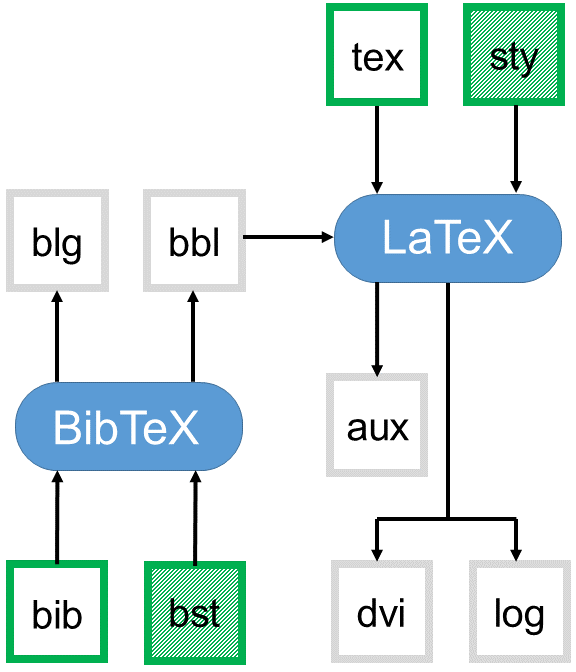
\includegraphics[scale=0.5]{LaTeX_diagram}
\caption{LaTeX diagram}
\label{fig:universe}
\end{figure}

\begin{equation}
\frac{d}{dt}=\int_0^\infty
\label{eq:integral}
\end{equation}

\section{Conclusion}
``I always thought something was fundamentally wrong with the universe'' \cite{FordVersypt:2014}

\bibliographystyle{plain}
\bibliography{references}
\end{document}
